%%%%%%%%%%%%%%%%%%%%%%%%%%%%%%%%%%%%%%%%%
% Short Three-Column Newsletter
% LaTeX Template
% Version 1.0 (11/9/13)
%
% Original author:
% Frits Wenneker (http://www.howtotex.com) 
% With extensive modifications by:
% Vel (vel@latextemplates.com)
% 
% This template has been downloaded from:
% http://www.LaTeXTemplates.com
%
% License:
% CC BY-NC-SA 3.0 (http://creativecommons.org/licenses/by-nc-sa/3.0/)
%
%%%%%%%%%%%%%%%%%%%%%%%%%%%%%%%%%%%%%%%%%

%----------------------------------------------------------------------------------------
%	PACKAGES AND DOCUMENT CONFIGURATIONS
%----------------------------------------------------------------------------------------

\documentclass[10pt,a4paper,ngerman,twoside]{article} % Paper type (a4paper, usletter or legal) and font size (10, 11 or 12)

%\setlength\topmargin{-80mm} % Top margin
\setlength\topmargin{-48pt} % Top margin
\setlength\headheight{0pt} % Header height
\setlength\textwidth{7.0in} % Text width
\setlength\textheight{9.5in} % Text height
\setlength\oddsidemargin{-30pt} % Left margin
\setlength\evensidemargin{-30pt} % Left margin (even pages) - only relevant with 'twoside' article option
%\setlength\inner{4cm}
%\setlenfth\outer{2cm}
%\usepackage{geometry}
%\geometry{bindingoffset=20mm}
%\setlength\bindingoffset{2cm}

\usepackage{charter} % Charter font for main content

\frenchspacing % Reduces space after periods to make text more compact for a three-column layout
\usepackage{babel}
\usepackage[utf8]{inputenc}
\usepackage{graphicx} % Required for including images
\usepackage{amssymb} % Math packages
\usepackage{amsmath} 
\usepackage{multicol} % Required for the three-column layout of the document
\usepackage{url} % Clickable links
\usepackage{enumitem} % Reduces the amount of space within and between lists with [noitemsep,nolistsep]
\usepackage{marvosym} % Required for the use of symbols
\usepackage{wrapfig} % Allows wrapping text around figures
%\usepackage[T1]{fontenc} % Use 8-bit encoding that has 256 glyphs
\usepackage{datetime} % Required for defining a custom date style
\newdateformat{mydate}{\monthname[\THEMONTH] \THEYEAR} % Set a custom date format
\usepackage[pdfpagemode=FullScreen, colorlinks=false]{hyperref} % Link colors and PDF behavior in Acrobat
\usepackage{fancyhdr} % Required to define custom headers/footers
\usepackage{hyperref} % funktioniert nicht ?
\pagestyle{fancy} % Enables the custom headers/footers for all pages following this

%-----------------------------------------------------------
% Header and footer
\lfoot{\footnotesize % Left footer containing newsletter contact information
%\begin{wrapfigure}{l}{2.0cm}
%
\includegraphics[width=2cm]{ccbysa88x31.png} 
%\end{wrapfigure}
R.I.S. Journal Ausgabe 001, Jänner 2014: \textbf{R}emix, \textbf{I}mprove, \textbf{S}hare. Das freie, creativ-commons lizensierte Journal.  \\
\Mundus\ Download und andere Formate: \href{http://spielend-programmieren.at/de:ris:start}{\texttt{spielend-programmieren.at/de:ris:start}} \quad
%\Telefon\ (000) 111-1111 \quad
\Letter\ \href{mailto:horst.jens@spielend-programmieren.at}{horst.jens@spielend-programmieren.at}
}

\cfoot{} % Empty center footer

\rfoot{\footnotesize ~\\ Seite \thepage} % Right footer - page counter

\renewcommand{\headrulewidth}{0.0pt} % No horizontal rule for the header
\renewcommand{\footrulewidth}{0.4pt} % Horizontal rule separating the footer from the document
%-----------------------------------------------------------

%-----------------------------------------------------------
% Define separators
\newcommand{\HorRule}[1]{\noindent\rule{\linewidth}{#1}} % Creates a horizontal rule
\newcommand{\SepRule}{\noindent	% Creates a shorter separator rule
\begin{center}
\rule{250pt}{1pt} % Page width and rule width
\end{center}
}
\newcommand{\Trenner}{\noindent
\begin{center}
\rule{100pt}{1pt}
\end{center}
}
%-----------------------------------------------------------

%-----------------------------------------------------------
% Define title and article styles
\newcommand{\NewsletterName}[1]{ % Newsletter title
\begin{center}
\Huge \usefont{T1}{fvs}{b}{n} % Use the Bera Sans Bold font
#1
\end{center}	
\par \normalsize \normalfont}

\newcommand{\JournalIssue}[1]{ % Date and issue number at the top of the newsletter
%\hfill \textsc{\mydate \today, No #1} % Right-aligned date and issue number
\hfill \textsc{Jänner 2014, Ausgabe 001}
\par \normalsize \normalfont}

\newcommand{\NewsItem}[1]{ % News item title
\usefont{T1}{fvs}{n}{n} % Use the Bera Sans Normal font
\vspace{24pt}\large #1\vspace{3pt} % Print the title with space around it in a larger font size
\par \normalsize \normalfont}

\newcommand{\NewsAuthor}[1]{ % Author name under the item title
\hfill von \textsc{#1} \vspace{20pt} % Right-aligned author name in small caps with space after it
\par \normalfont}		

%----------------------------------------------------------------------------------------
%	TITLE
%----------------------------------------------------------------------------------------

\begin{document}

\JournalIssue{1} % Issue number
\NewsletterName{R.I.S. Journal} % Newsletter title
%\begin{center}
%\textbf{R}emix \textbf{I}mprove \textbf{S}hare - das freie Journal für Open Source Education
%\end{center}
\noindent\HorRule{3pt} \\[-0.75\baselineskip] % Thick horizontal rule
\HorRule{1pt} % Thin horizontal rule



%\setlength{\columnsep}{16pt} % Uncomment to manually change the white space between columns
%\begin{multicols}{3} % Begin the three-column layout

%----------------------------------------------------------------------------------------
%	OTHER NEWS
%----------------------------------------------------------------------------------------
%-----------------------------------------------------------
%
%-----------------------------------------------------------
%RIS-Journal Titel (Titelgrafik hier einfügen)
%start splitting here
%---------------------------------------------------------
\begin{center}
%
\includegraphics[width=0.9\linewidth]{austrianguy/austrianguy.png}
\textbf{R}emix \textbf{I}mprove \textbf{S}hare - das freie, creative-commons lizensierte Journal zu den Themen Open-Source, Spiele Programmierung, Open Education. \textbf{Preis:} Zahlen Sie so viel Sie wollen (siehe Bitcoin- und Flattr-QR-Code).
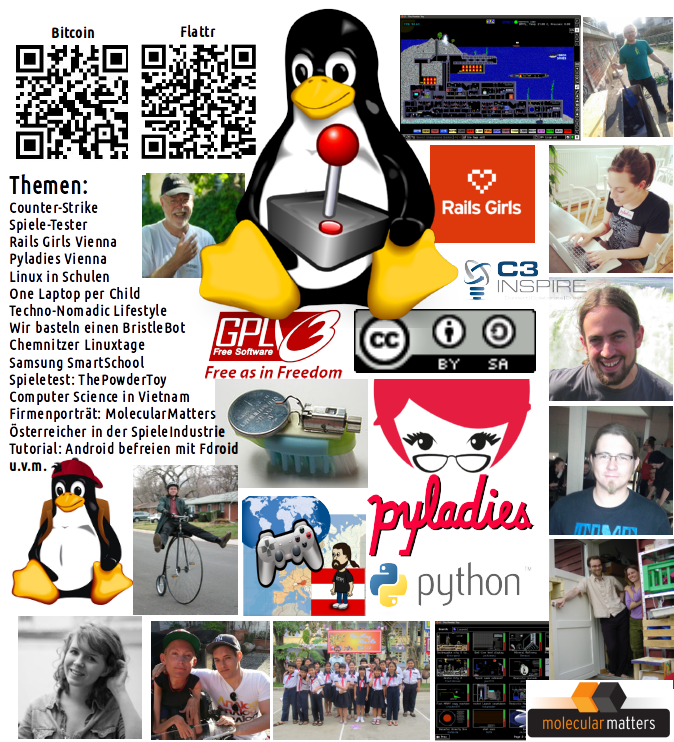
\includegraphics[width=\linewidth]{titelbild.png}
\end{center}
%---------------------------------------------------------
\begin{multicols}{3}
\NewsItem{}
\section*{Inhalt} 
\label{inhalt}

\textbf{Impressum}: \texttt{impressum, S. \pageref{impressum}}\\
\textbf{Editorial}: Horst Jens (Herausgeber) über den Zweck dieser Zeitschrift, Creative-Commons Lizenzen und Free Software culture: \texttt{editorial, S. \pageref{editorial}}\\ 
\textbf{Kalender}: Termine für 2014: \texttt{kalender, S. \pageref{kalender}}

\subsection*{Report}

\textbf{Linuxtage} 2013 in Chemnitz, Vortrag über Linux in Schulen, OSDomotics Smarthome: \texttt{chemnitz, S. \pageref{chemnitz}}\\

\subsection*{Lifestyle}

\textbf{Freiwillig obdachlos}: \texttt{nomad, S. \pageref{nomad}}\\
\textbf{Billionär werden}: \texttt{trilions, S. \pageref{trillions}}\\

\subsection*{Beruf}

\textbf{Berufsbild: Spiele Tester}: \texttt{spieletester, S. \pageref{spieletester}}\\
\textbf{Firmengründer} Stefan Reinalter erzählt über seine Spielegrafik-Engine: \texttt{molecularmatters, S. \pageref{molecularmatters}}\\
\textbf{Lebensweg}: Wie ein Österreicher seinen Weg in die games industry fand: \texttt{austrianguy, S. \pageref{austrianguy}}\\
\textbf{Berufsbild: Counterstrike-Profispieler}: \texttt{counterstrike, S. \pageref{counterstrike}}\\
\textbf{Warnung}: Meide die Games Industry ! (Rant auf reddit.com): \texttt{redditrant, S. \pageref{redditrant}}\\

\subsection*{Schule}

\textbf{Meinung}: Wie smart ist die Samsungs Smartschool ? \texttt{smartschool, S. \pageref{smartschool}}\\
\textbf{Kanada}: c3inspire bringt Studierende von Technik und Wirtschaft zusammen: \texttt{c3inspire, S. \pageref{c3inspire}}\\
\textbf{England}: Umstellung einer Mädchenschule auf Linux: \texttt{westcliff, S. \pageref{westcliff}}\\
\textbf{USA / Vietnam}: Neil Fraser macht in \textbf{Vietnam} Urlaub, erforscht den Computer Science Unterricht vor Ort und prgrammiert ein grafisches Lerntool: \texttt{vietnam, S. \pageref{vietnam}}\\ 
\textbf{OLPC Austria}: Christoph Derndofer macht sich Gedanken über das \textbf{One Laptop per Child} Projekt: \texttt{olpcnewyear, S. \pageref{olpcnewyear}}\\

\subsection*{Mädchen programmieren}

\textbf{Pyladies Vienna} Gründerin \textit{Floor Drees} im Interview \texttt{floor, S. \pageref{floor}}\\
\textbf{Railsgirls} haben mein Leben verändert: Blogposting von \textit{Laura Gaetano} über Railsgirls, Pyladies und wie man Schriftstellerin wird: \texttt{laura, S.\pageref{laura}}\\

\subsection*{Praxis}

\textbf{Tutorial}: Freies Software-Repository für \textbf{fdroid} für Android installieren: \texttt{fdroid, S. \pageref{fdroid}}\\ \textbf{Hardware}: Tutorial: \textbf{Zahnbürsten-Roboter} selber machen: \texttt{bristlebot, S. \pageref{bristlebot}}\\

\subsection*{Game}

\textbf{Open Source game}: Chemiebaukasten: Welten zerstören mit \textbf{The Powder Toy}: \texttt{powdertoy, S. \pageref{powdertoy}}\\
\textbf{Tutorial}: Wasser bewegen mit The Powder Toy: \texttt{powdertoytutorial, S. \pageref{powdertoytutorial}}\\
\textbf{Tutorial}: Ballspiel grafisch programmieren mit \textbf{Scratch2}: \texttt{scratch, S. \pageref{scratch}}\\
\end{multicols}
%---------------------------------------------------------
\SepRule % weil auf selber Seite
\begin{multicols}{3}
\NewsItem{}
\section*{Inhalt} 
\label{inhalt}

\textbf{Impressum}: \texttt{impressum, S. \pageref{impressum}}\\
\textbf{Editorial}: Horst Jens (Herausgeber) über den Zweck dieser Zeitschrift, Creative-Commons Lizenzen und Free Software culture: \texttt{editorial, S. \pageref{editorial}}\\ 
\textbf{Kalender}: Termine für 2014: \texttt{kalender, S. \pageref{kalender}}

\subsection*{Report}

\textbf{Linuxtage} 2013 in Chemnitz, Vortrag über Linux in Schulen, OSDomotics Smarthome: \texttt{chemnitz, S. \pageref{chemnitz}}\\

\subsection*{Lifestyle}

\textbf{Freiwillig obdachlos}: \texttt{nomad, S. \pageref{nomad}}\\
\textbf{Billionär werden}: \texttt{trilions, S. \pageref{trillions}}\\

\subsection*{Beruf}

\textbf{Berufsbild: Spiele Tester}: \texttt{spieletester, S. \pageref{spieletester}}\\
\textbf{Firmengründer} Stefan Reinalter erzählt über seine Spielegrafik-Engine: \texttt{molecularmatters, S. \pageref{molecularmatters}}\\
\textbf{Lebensweg}: Wie ein Österreicher seinen Weg in die games industry fand: \texttt{austrianguy, S. \pageref{austrianguy}}\\
\textbf{Berufsbild: Counterstrike-Profispieler}: \texttt{counterstrike, S. \pageref{counterstrike}}\\
\textbf{Warnung}: Meide die Games Industry ! (Rant auf reddit.com): \texttt{redditrant, S. \pageref{redditrant}}\\

\subsection*{Schule}

\textbf{Meinung}: Wie smart ist die Samsungs Smartschool ? \texttt{smartschool, S. \pageref{smartschool}}\\
\textbf{Kanada}: c3inspire bringt Studierende von Technik und Wirtschaft zusammen: \texttt{c3inspire, S. \pageref{c3inspire}}\\
\textbf{England}: Umstellung einer Mädchenschule auf Linux: \texttt{westcliff, S. \pageref{westcliff}}\\
\textbf{USA / Vietnam}: Neil Fraser macht in \textbf{Vietnam} Urlaub, erforscht den Computer Science Unterricht vor Ort und prgrammiert ein grafisches Lerntool: \texttt{vietnam, S. \pageref{vietnam}}\\ 
\textbf{OLPC Austria}: Christoph Derndofer macht sich Gedanken über das \textbf{One Laptop per Child} Projekt: \texttt{olpcnewyear, S. \pageref{olpcnewyear}}\\

\subsection*{Mädchen programmieren}

\textbf{Pyladies Vienna} Gründerin \textit{Floor Drees} im Interview \texttt{floor, S. \pageref{floor}}\\
\textbf{Railsgirls} haben mein Leben verändert: Blogposting von \textit{Laura Gaetano} über Railsgirls, Pyladies und wie man Schriftstellerin wird: \texttt{laura, S.\pageref{laura}}\\

\subsection*{Praxis}

\textbf{Tutorial}: Freies Software-Repository für \textbf{fdroid} für Android installieren: \texttt{fdroid, S. \pageref{fdroid}}\\ \textbf{Hardware}: Tutorial: \textbf{Zahnbürsten-Roboter} selber machen: \texttt{bristlebot, S. \pageref{bristlebot}}\\

\subsection*{Game}

\textbf{Open Source game}: Chemiebaukasten: Welten zerstören mit \textbf{The Powder Toy}: \texttt{powdertoy, S. \pageref{powdertoy}}\\
\textbf{Tutorial}: Wasser bewegen mit The Powder Toy: \texttt{powdertoytutorial, S. \pageref{powdertoytutorial}}\\
\textbf{Tutorial}: Ballspiel grafisch programmieren mit \textbf{Scratch2}: \texttt{scratch, S. \pageref{scratch}}\\
\end{multicols}
%\SepRule

%-----------------------------------------------------------
\end{document}
